\documentclass[]{spie}  %>>> use for US letter paper
%\documentclass[a4paper]{spie}  %>>> use this instead for A4 paper
%\documentclass[nocompress]{spie}  %>>> to avoid compression of citations

\renewcommand{\baselinestretch}{1.0} % Change to 1.65 for double spacing

\usepackage{amsmath}
\usepackage{amsfonts}
\usepackage{amssymb}
\usepackage{graphicx}
\usepackage[caption = false]{subfig}
\usepackage[colorlinks=true, allcolors=blue]{hyperref}
\usepackage{mwe}
\usepackage{todonotes}
\usepackage{siunitx}

\DeclareSIUnit\milliarcsecond{mas}

% Option to view page numbers
\pagestyle{plain} % change to \pagestyle{plain} for page numbers

%%%%% Authors %%%%%

\title{A Visible-light Lyot Coronagraph for SCExAO/VAMPIRES}

\author[a,*]{Miles Lucas}
\author[a]{Michael Bottom}
\author[b,c]{Olivier Guyon}
\author[b]{Julien Lozi}
\author[d]{Barnaby Norris}
\affil[a]{Institute for Astronomy, Unviersity of Hawai'i,  640 N. Aohoku Pl., Hilo, HI 96720, USA}
\affil[b]{National Observatory of Japan, Subaru Telescope, 650 N. Aohoku Pl., Hilo, HI 96720, USA}
\affil[c]{Steward Observatory, Unviersity of Arizona, 933 N. Cherry Ave., Tucson, AZ 85721, USA}
\affil[d]{Sydney Institute for Astronomy, School of Physics, Physics Rd., University of Sydney, NSW 2006, Australia}

\authorinfo{Further author information: (Send correspondence to M.L.)\\M.L.: E-mail: mdlucas@hawaii.edu}

\begin{document}
\maketitle

%%%%% Abstract %%%%%

\begin{abstract}
   We describe the design and initial results from a visible-light Lyot coronagraph for SCExAO/VAMPIRES. The coronagraph comprises four hard-edged, partially transmissive focal plane masks with inner working angles of \qtylist{36;55;92;129}{\milliarcsecond}, respectively. The Lyot stop is a reflective, undersized design with a relative throughput of 65.7\%. Our preliminary on-sky contrast is \num{e-2} at \ang{;;0.1} to \num{e-4} at \ang{;;0.75} for all mask sizes. The coronagraph was deployed in early 2022 and has been approved for open-use.
\end{abstract}

%%%%% Keywords %%%%%

\keywords{Coronagraph, Optical, Visible, High-Contrast, Imaging, Exoplanets}

%%%%% Main body %%%%%

\section{Introduction}\label{sec:intro}


In recent decades exoplanet science has advanced tremendously, with over \num{5,000} confirmed planets orbiting a variety of stars in our galaxy\cite{akeson2013}. These planets have predominantly been discovered and characterized using the indirect methods of transit photometry or radial velocity analysis\cite{perryman2018}. Direct imaging, or high-contrast imaging, probes a complenetary phase space of exoplanets while providing direct observations of exoplanets. In order to accomplish this, a combination of high-performance instrumentation, observational techniques, and post-processing methods must be employed. In the past few years, high-contrast instruments like SPHERE\cite{petit2014}, GPI\cite{macintosh2014}, and SCExAO\cite{jovanovic2015a} have greatly advanced the field of direct imaging. These instruments typically operate in the near-infrared (near-IR), from Y to L band, for two reasons. First is for the increased brightness of thermal emission of exoplanets in the near-IR, which lowers the relative flux ratio between the star and the exoplanet (contrast), ultimately improving the detection sensitivity to smaller planets. Second, in the near-IR wavefront control with adaptive optics (AO) is more powerful than the optical. This is because  the same path length error is a smaller phase error in the near-IR than the visible, simply due to the wavelength difference.

Despite the challenges of high-performance, diffraction limited imaging in the visible, there are significant motivations for extending high-contrast imaging into the optical. First, consider the detection of reflected-light from exoplanets, which is considered the most promising method of imaging terrestrial planets\cite{traub2010}. Second, an important component of improving planet-formation theory is studying the birth of exoplanets in protoplanetary disks, which can be imaged using light reflected from small dust grains suspended in the gas disk. Such observations of protoplanetary disks are very complementary to the radio imaging of the debris, and probe smaller angles, better angular resolutions, and different grain chemistries than near-IR reflected light imaging. Lastly, using H$\alpha$ emission (\qty{656.28}{\nano\meter}) as a tracer for accretion allows direct imaging of matter accreting onto forming exoplanets\cite{currie2022}, as well as studying mass-loss in giant stars\cite{norris2020}.

The Visible Aperture-Masking Polarimetric Interferometer/Imager for Resolving Exoplanetary Signatures (VAMPIRES)\cite{norris2015} is an optical dual-beam imager for the Subaru Coronagraphic Extreme Adaptive Optics (SCExAO) instrument on the Subaru telescope. VAMPIRES operates between \qtyrange{600}{800}{\nano\meter} with capabilities for polarimetric imaging\cite{norris2020}, H$\alpha$ imaging\cite{uyama2020}, and focal plane wavefront sensing\cite{vievard2020}. VAMPIRES also has a suite of non-redundant sparse aperture masks for sub-diffraction-limited interferometric imaging of stellar surfaces and outflows. For this work, though, we will focus on the traditional and polarimetric imaging modes.

VAMPIRES currently uses two Andor electron-multiplying (EM) CCDs for low readnoise with framerates from \qtyrange{1}{100}{\hertz}. While these detectors perform very well in the photon-limited regime, the strong non-linearities and compressed dynamic range from electron multiplication makes imaging bright targets ($m^I < 7$) difficult. In order to address this problem, we have designed and deployed a classic Lyot coronagraph (CLC), which greatly attenuates the stellar point spread function (PSF), allowing use of high EM gain without saturation. This is the primary motivation for building a coronagraph for VAMPIRES- avoiding saturation is key for CCD imaging, but this limits the off-axis signal to noise ratio (S/N). By attenuating the on-axis light, the off-axis signal can be increased without saturation from the stellar PSF, ultimately improving the S/N.

Furthermore, coronagraphy improves the detection sensitivity of in circumstellar regions by controlling the stellar diffraction pattern. In other words, the coronagraph does not simply mask the central region of the image, but rather attenuates the effects of the stellar PSF throughout the entire field of view (FOV). The diffraction control of a coronagraph is highly dependent on the quality of the incoming wavefront, though, necessitating the use of AO for high-contrast imaging. When combined with extreme AO, such as provided by SCExAO, a coronagraph can enable detections of sources many orders of magnitude fainter than their host stars ($\sim$\num{e-6})\cite{guyon2018}.

This report details our design and deployment of a visible-light coronagraph for VAMPIRES. In \autoref{sec:methods} we detail our modeling and simulation of the coronagraph and the construction of the optics. In \autoref{sec:tests} we describe our characterization of the coronagraph, including throughput and inner working angle. Finally, in \autoref{sec:results} we discuss the performance of the coronagraph with the calibration light source and on sky.

\section{Methods}\label{sec:methods}

\subsection{Designing the Coronagraph}\label{sec:design}

We used the open-source python package \texttt{HCIPy}\cite{por2018} for simulating our coronagraph design with Fourier optics. We defined our wavefronts on a rasterized image of the SCExAO pupil sampled on a 256x256 pixel grid (\autoref{fig:pupil}a). Initially, we do not introduce any wavefront errors. Using a Fraunhofer propagator with an F/28.4 focal ratio, we formed the intermediate focal plane, where the focal plane mask will be inserted. VAMPIRES has a FOV of \ang{;;3}x\ang{;;3}, however, for our exploratory simulations we only calculated the first 16 airy rings (\autoref{fig:pupil}b). The focal plane masks are hard-edged circles, and were modeled using a circular apodizer with either 0\% or 0.1\% transmission. We designed four focal plane masks with radii of \qtylist{38.6;57.9;96.5;135}{\micro\meter}, respectively. These radii correspond to \numlist{2;3;5;7} $\lambda/D$ at \qty{750}{\nano\meter}, or \qtylist{35.9;53.9;89.8;126}{\milliarcsecond}. The focal plane after the mask was propagated to the next pupil plane, where the Lyot stop apodized the wavefront.

\begin{figure*}
   \centering
   \includegraphics[width=\textwidth]{figures/aperture_psf}
   \caption{(a) The SCExAO pupil, which is slightly undersized compared to the Subaru aperture and contains additional features. The aperture diameter is 95\% of the Subaru clear aperture; effectively \qty{7.79}{\meter}. The central obstruction is 31\% of this diameter. The two additional circles are masks for inactive deformable mirror actuators, one of which lies on a spider segment, while the other requires an additional spider. (b) The VAMPIRES PSF simulated using \texttt{HCIPy}. The four grayscale circles correspond to the focal plane mask sizes.}\label{fig:pupil}
\end{figure*}

The Lyot stop was modeled using a series of circular and rectangular apodizers with 0\% transmission. The stop design follows the shape of the SCExAO pupil with an undersized diameter and oversized obstructions. The outer diameter is 90\% the clear aperture diameter, the inner obstruction is 45\% the clear aperture diameter, the secondary support struts are 200\% their original width, and the bad deformable mirror probes are 150\% oversized. The ratio of areas of the Lyot stop and the SCExAO pupil is 63.7\%, and will theoretically widen the diffraction limit by 10\%. This final wavefront was propagated to the detector focal plane, forming the post-coronagraphic point-spread function.

We repeated the above process for a series of wavelengths to approximate a broadband PSF. We summed the images produced with 10 wavefronts from \qtyrange{725}{775}{\nano\meter} to mimic the ``750-50'' filter (\qty{750}{\nano\meter} central wavelength with \qty{50}{\nano\meter} uniform bandpass). We chose this filter because at these wavelengths VAMPIRES has the highest throughput and best polarimetric efficiency. As an additional step, we generated many datasets with random tip and tilt errors sampled from a bivariate Gaussian with \qty{10}{\milliarcsecond} root-mean-square (RMS) jitter to test the coronagraph's resiliency to low-order wavefront errors. SCExAO typically has higher RMS tip-tilt error than \qty{10}{\milliarcsecond}, which is actually closer to the 90th-percentile of on-sky performance. However, since VAMPIRES often operates in high-framerate lucky imaging mode, the effects of tip-tilt can be mitigated.

We evaluated the performance and quality of our simulations from the raw contrast curves of each mask \autoref{fig:sim-contrast}. These curves measure the noise in concentric annuli around the PSF. Each annulus is one full-width at half-maximum (FWHM) wide, and the noise is calculated using the biweight scale, which is robust to outliers such as cosmic rays. The noise estimate also takes into account small-sample statistics\cite{mawet2014}, which biases the noise measured in annuli close to the PSF. We take the radial profile of this noise and normalize it to the non-coronagraphic PSF flux to determine the raw contrast, where we then apply a 5$\sigma$ detection threshold. For clarity, we describe all our contrast curves as ``raw'' since we never do PSF subtraction in this work. To create these contrast curves We used the open-source package \texttt{ADI.jl}\cite{lucas2020}.

\begin{figure*}
   \centering
   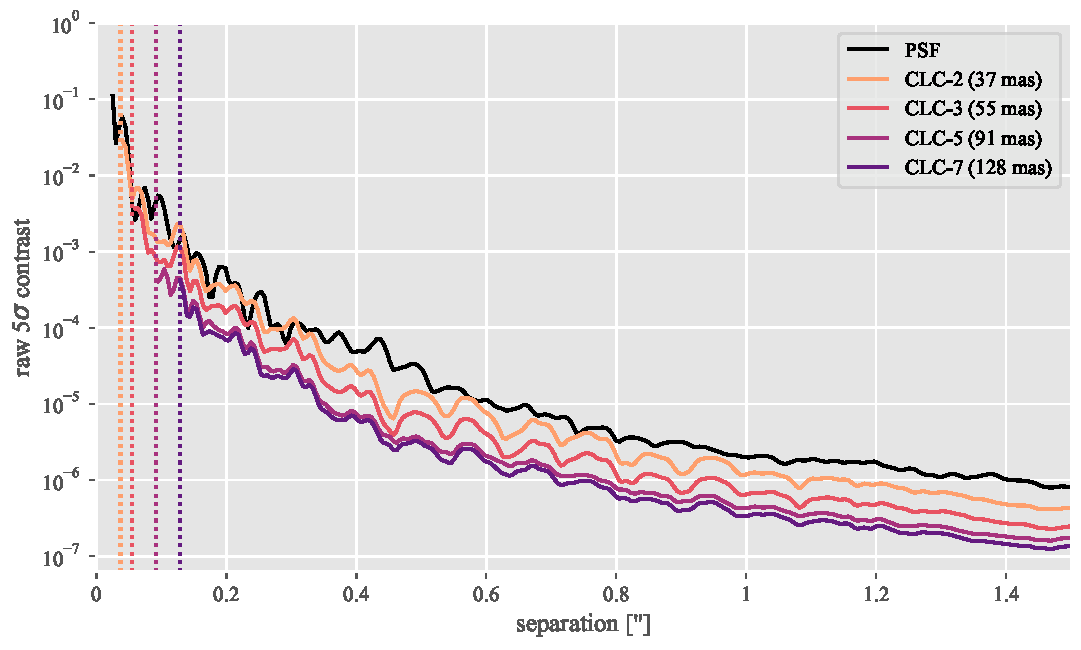
\includegraphics[width=0.95\textwidth]{figures/simulated_curves}
   \caption{Simulated raw 5$\sigma$ contrast curves for an unocculted PSF (black line) and for each focal plane mask size (orange to purple lines). These curves are calculated from images simulated with \texttt{HCIPy}. The mask inner working angles are marked by vertical dotted lines}\label{fig:sim-contrast}
\end{figure*}

From the raw contrast curves, we found that the CLC-2 mask does not attenuate the PSF that well, especially at close angles ($<$\ang{;;0.4}). The CLC-3 mask only offers a factor of a few improved contrast compared to the unocculted PSF. We found no significant performance differences between the CLC-5 and CLC-7 masks, both showing an improvement of an order of magnitude of sensitivity throughout the FOV. The typical read noise and non-common path wavefront errors in VAMPIRES are expected to ultimately limit our contrast at large separations. As we will describe in \autoref{sec:install}, the focal plane masks are diced from a single piece of glass producing four substrates. So we decided to construct all four mask sizes with two variations each: one partially transmissive (0.1\%) and the other fully opaque.

\subsection{Construction and Installation}\label{sec:install}

We used a metallic vapor deposition process (\url{https://opto-line.com/}) for applying the focal plane mask and Lyot stop patterns to our substrates. The metals are deposited onto a glass substrate with micrometer-precision, giving us great flexibility and precision in our design patterns and the thickness of the material. One downside of this approach is that the glass focal plane mask will shift the focus since it is located in a converging beam. In VAMPIRES, there is a custom optics mount in the focal plane with \qty{8}{\milli\meter} x \qty{8}{\milli\meter} slots, so we arranged for four masks to be diced from a single \qty{30}{\milli\meter} anti-reflection (AR) coated optical flat (\href{https://www.edmundoptics.com/p/30mm-dia-4mm-thick-nir-i-coated-lambda10-fused-silica-window/27562/}{Edmund Optics \#84-466}), making sure each segment was within the clear aperture. The focal plane mask dots were deposited using chromium with a thicknesses of \qtylist{110;300}{\nano\meter}. The thickness was determined from the optical penetration depth for a desired transmission
\begin{equation}
    \hat{s}(\lambda) = -\frac{\lambda}{4\pi\tilde{k}(\lambda)}\ln{\frac{I(\lambda)}{I_0(\lambda)}}
    \label{eqn:throughput}
\end{equation}
where $\hat{s}$ is the thickness, $\lambda$ is the wavelength (tested across the 600-800 nm range for VAMPIRES), $\tilde{k}$ is the extinction coefficient, and $I/I_0$ is the relative intensity for transmitted light. The thicknesses of \qtylist{110;300}{\nano\meter} correspond to transmissions of \num{e-1} and \num{e-8}, respectively, matching our design goals of 0.1\% and 0\%.

The Lyot stop pattern was deposited onto a \qty{25}{\milli\meter} AR-coated optical flat (\href{https://www.edmundoptics.com/p/25mm-dia-3mm-thick-nir-i-coated-lambda10-fused-silica-window/27561/}{Edmund Optics \#84-465}) with no further processing. We chose a reflective gold coating which allows easy mask alignment with VAMPIRES' pupil camera. Following advice from our vendor, this gold layer was deposited on top of a layer of chromium, which adheres better to AR coatings than gold. We used \autoref{eqn:throughput} to determine a combined thickness of \qty{285}{\nano\meter} for \num{e-8} transmission. The final thickness of the chromium and gold deposit was specified as \qty{300}{\nano\meter}.

\begin{figure*}
   \centering
   \subfloat{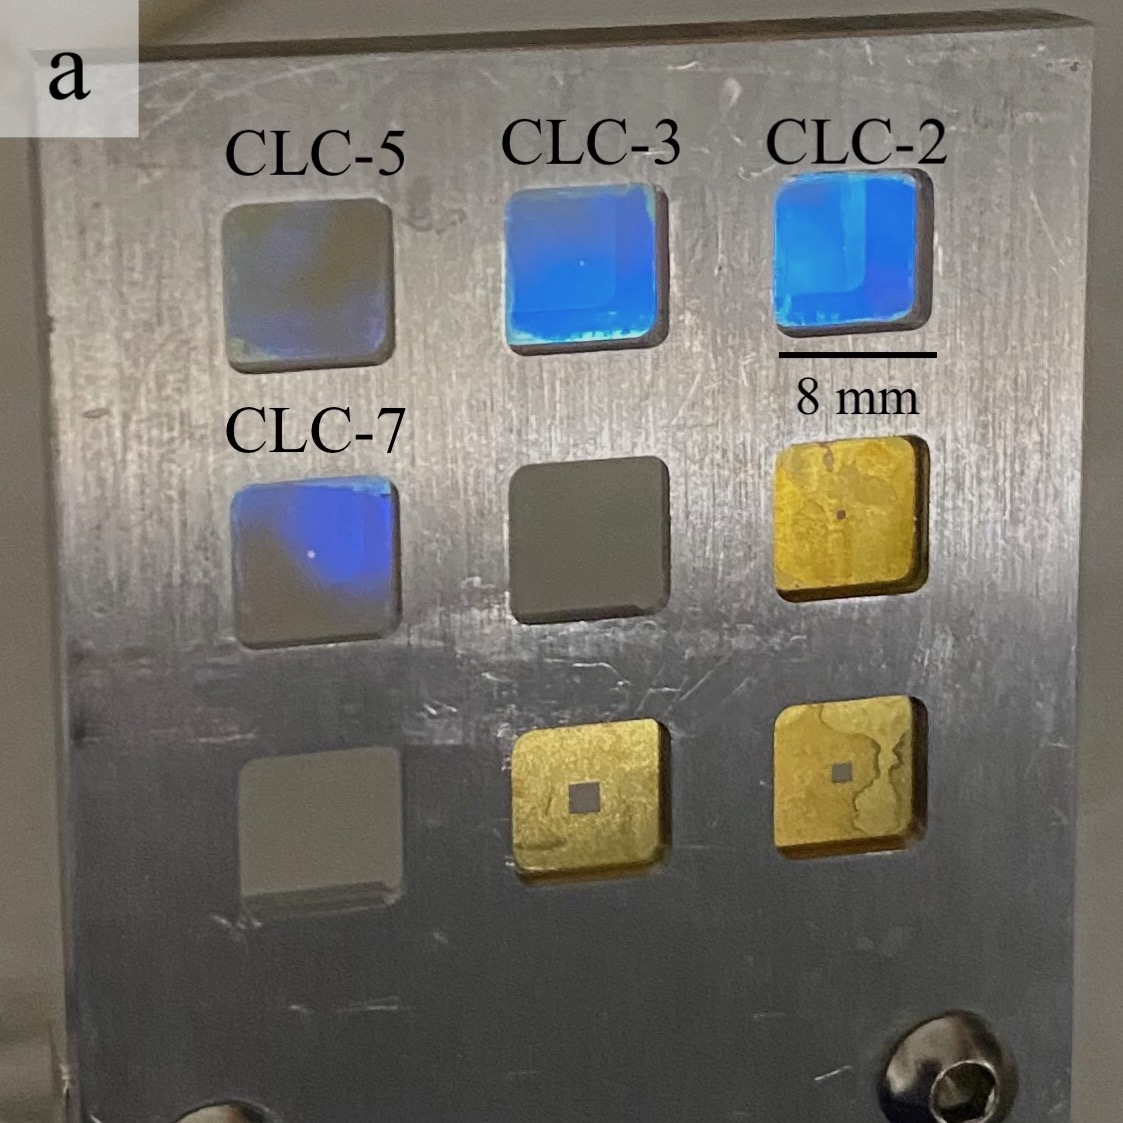
\includegraphics[width=2.5in]{figures/fpm.jpeg}}\hspace{0.5in}
   \subfloat{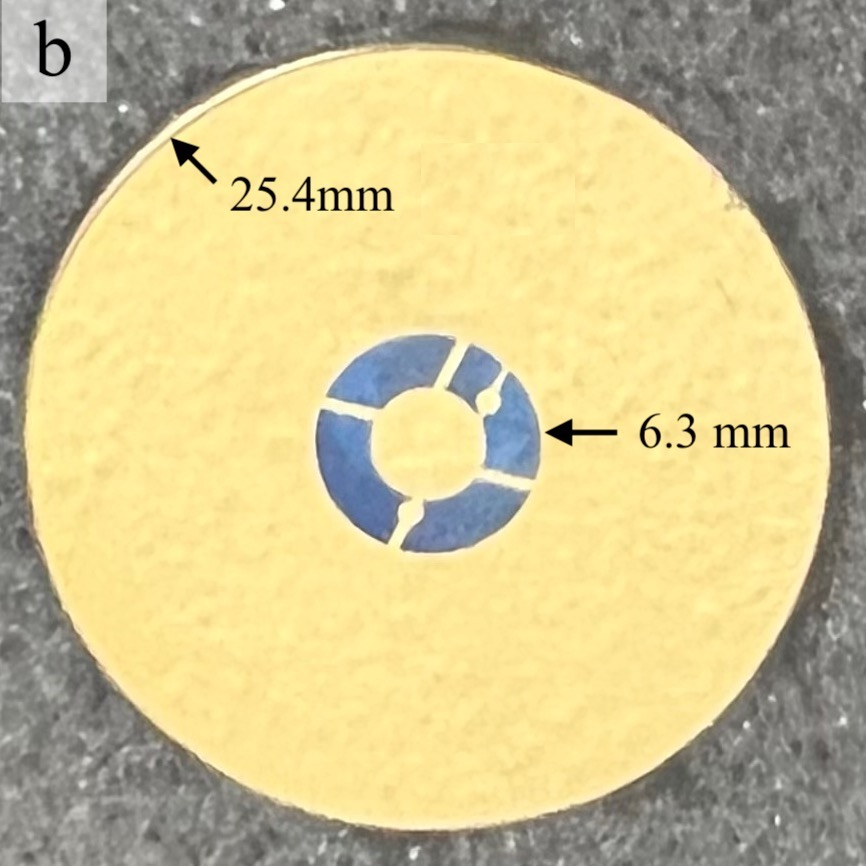
\includegraphics[width=2.5in]{figures/lyot_stop.jpeg}}
   \caption{(a) The four focal plane masks mounted in the custom-machined focal plane mount for VAMPIRES. The size of each slot is \qty{8}{\milli\meter}x\qty{8}{\milli\meter}. (b) The undersized Lyot stop with its reflective gold coating. The diameter of the glass substrate and stop outer diameter are marked.}\label{fig:optics}
\end{figure*}

\section{Operation and Characterization}\label{sec:tests}

Both the focal plane masks and Lyot stop are installed in mounts with precise motor controllers for alignment. We found that the Lyot stop, being in the collimated beam, stays consistently aligned in-between instrument cranings. The focal plane masks take around a minute to manually align and focus.

\subsection{Artifical Calibration Speckles (``Astrogrid'')}

A common problem with coronagraphic imaging is accurately determing the flux and position of the host star while behind the focal plane mask. By adding sinusoidal patterns to the deformable mirror (DM) copies of the stellar PSF will appear off-axis depending on the frequency of the sinusoidal pattern\cite{sahoo2020}. These patterns are modulated in two ways: first the patterns are modulated spatially by half a wavelength to average effects of atmospheric seeing on the speckles during a typical integration. Second, the pattern is spatially modulated to create alternating sets of two PSFs, for a total of four calibration speckles equidistant from the star. The brightness of these ``satellite spots'' is proportional to the amplitude of the DM perturbation, which can be calibrated to give accurate relative photometry between the spots and the star. This method has been successfully demonstrated on SCExAO/CHARIS with astrometric precision $\sim$\qty{1.7}{\milliarcsecond} and photometric precision $\sim$0.3\%\cite{currie2020}. Examples of the ``astrogrid'' on VAMPIRES are shown in \autoref{fig:satellite-spots}.

\begin{figure*}
   \centering
   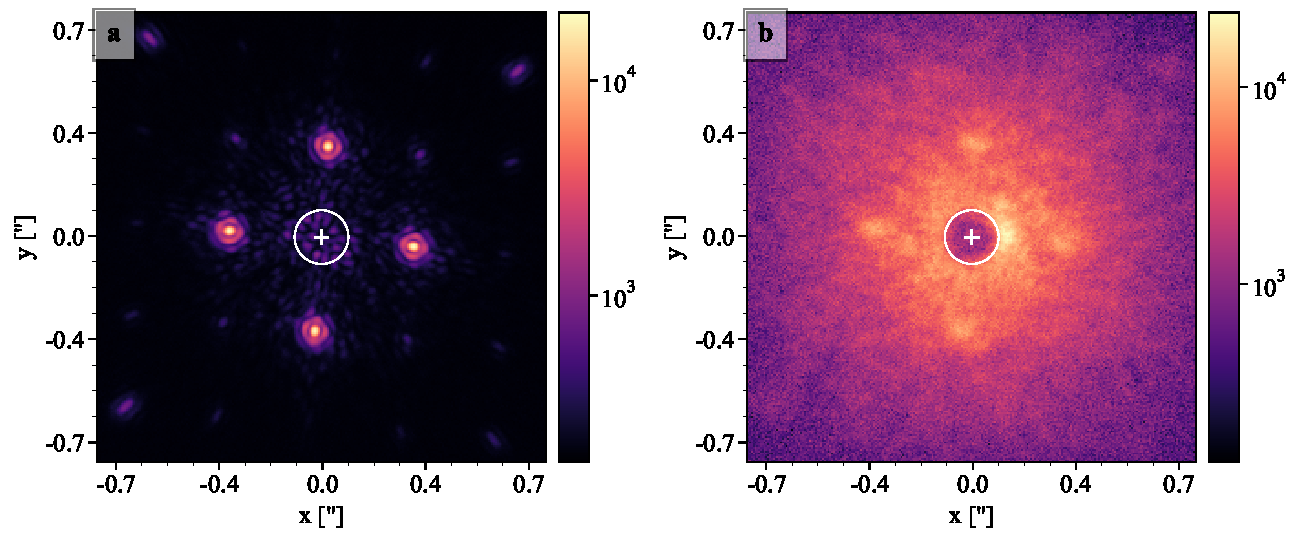
\includegraphics[width=\textwidth]{figures/astrogrid_psf}
   \caption{Coronagraphic images using the CLC-5 mask (\qty{91}{\milliarcsecond} IWA) with \qty{50}{\nano\meter} ``astrogrid'' calibration speckles. (a) A single frame of testbed data using the internal calibration source through the 750-50 filter with 110 EM gain, and \qty{20}{\milli\second} exposure length. (b) On-sky data of HIP 56083 from May 25, 2022 in poor seeing ($\sim$\ang{;;1.6}), using the 750-50 filter, 300 EM gain, and \qty{200}{\milli\second} exposure length.}\label{fig:satellite-spots}
\end{figure*}

\subsection{Coronagraphic throughput}

We measured both the relative Lyot stop throughput as well as the off-axis focal plane throughput for our coronagraph. The Lyot stop throughput is proportional to the unobstructed area of the mask compared to the pupil. From the drawings, the ratio of areas is 63.7\%. We measured the throughput using the pupil-imaging camera with the calibration light source, comparing the total intensity measured with a mirror in the pupil wheel (100\% of the incident light) versus the Lyot stop (blocked light only). We calculated a relative throughput of 65.7\%.

The off-axis coronagraphic throughput was measured by gradually moving the focal plane mask off-axis from the calibration source. The fluxes from all of the images were normalized so the maximum off-axis flux was 1 and the on-axis flux was 0 (\autoref{fig:throughput}). The inner working angle (IWA) is defined at 50\% throughput. The IWAs for each mask were interpolated from the data as \qtylist{36;55;92;129}{\milliarcsecond}, respectively, which is in good agreement with the radii of the masks.


\begin{figure*}
   \centering
   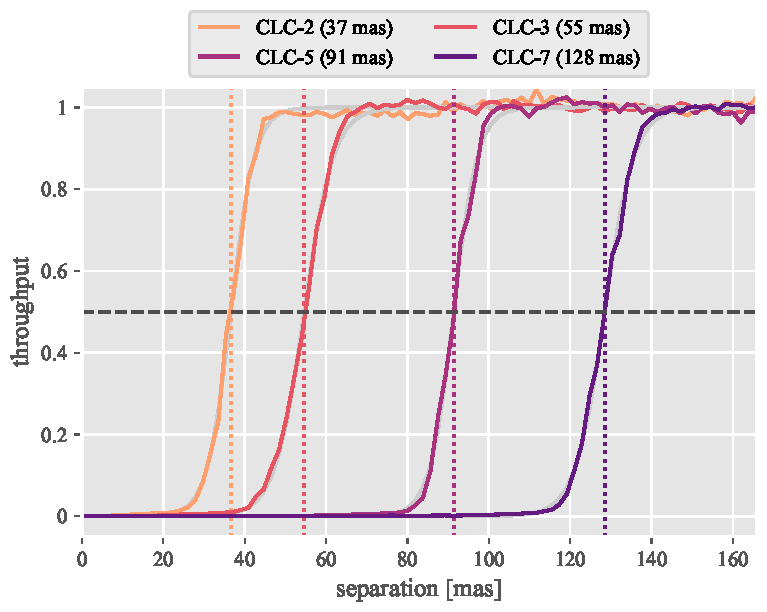
\includegraphics[height=4in]{figures/throughput_curves}
   \caption{Off-axis coronagraphic throughput for each focal plane mask. The flux throughput is normalized between 0 and 1. 50\% throughput is marked with a black dashed line and the inner working angles are denoted by the orange to purple dotted lines.}\label{fig:throughput}
\end{figure*}

\section{Results}\label{sec:results}

\subsection{Testbed results}\label{sec:testbed}

Our first tests use the calibration source on SCExAO for determining the contrast of the coronagraph for each focal plane mask. For these tests we used the 750-50 filter since it has the highest throughput. In addition, for all tests we applied an astrogrid with \qty{50}{\nano\meter} amplitude and a spatial frequency of 15.5 $\lambda/D$ (\qty{308}{\milliarcsecond}).

First, we took non-coronagraphic data allowing us to characterize both the photometry and astrometry of the astrogrid speckles as well as giving a non-coroangraphic PSF for measuring the relative attenuation of the coronagraph. For data reduction, we median-combined a series of 100 images and recentered the frame using the satellite spot centers of mass. For the astrogrid calibration, we used a hierarchical model of five two-dimensional Moffat functions
\begin{equation}
   \label{eqn:moffat}
   f\left( x, y | x_0, y_0, \Gamma, \alpha, I_0\right) = I_0 \left[1 + \frac{\left(x-x_0\right)^2 + \left(y-y_0\right)^2}{\Gamma^2} \right]^{-\alpha}
\end{equation}
where $(x_0, y_0)$ is the center of the PSF, $I_0$ is the peak amplitude, $\Gamma$ is the half-width at half-maximum (HWHM), and $\alpha$ is the exponential scaling factor, typically around 1 to 3. In our hierarchical model each PSF shares the $\Gamma$ and $\alpha$ parameters, and each of the four satellite spots share an amplitude. Around each PSF we measured the photometry using circular apertures with background subtraction from annular apertures. We measured the relative photometry of the \qty{50}{\nano\meter} amplitude astrogrid as $10^{-1.52}$.

Then we inserted the focal plane mask and Lyot stop and refocused. Again, we median-combined a series of 100 images and recentered using the satellite spots. To measure the photometry we fit a hierarchical model of four two-dimensional Moffat functions (\autoref{eqn:moffat}). This follows the same procedure as above with shared shape parameters and intensities, but this time without the on-axis PSF. Then, we measured the photometry of each satellite spot using circular apertures with an annulus for background subtraction. The stellar flux is estimated by the median flux of the four satellite spots scaled by the relative photometry fit above ($10^{-1.52}$).

From here we create raw contrast curves the same way as in \autoref{sec:design}, calculating the 5$\sigma$ detection limits (accounting for small-sample statistics) without PSF subtraction. Because we are not performing any kind of differential imaging, the satellite spots heavily bias the contrast, so we masked out the satellite spots during the noise calculations.

From the raw contrast curves (\autoref{fig:contrast}), we note similar performance between all the mask sizes. At \ang{;;0.1}, the coronagraph achieves a raw contrast of $\sim$ \num{e-3}, and a read-noise limited contrast beyond \ang{;;0.8} of $\sim$\num{e-5}. There is a large bump around the location of the satellite spots ($\sim$\ang{;;0.3}) and, to a lesser extent, around the secondary spots ($\sqrt{2}\cdot r \sim$ \ang{;;0.42}). Even with the masking, these spots are biased, we believe due to speckle pinning\cite{bloemhof2004}. We note that throughout the entire FOV the coronagraphs consistently attenuate the light by 1 to 1.5 orders of magnitude, addressing the dynamic range problems currently faced by VAMPIRES.


\begin{figure*}
   \centering
   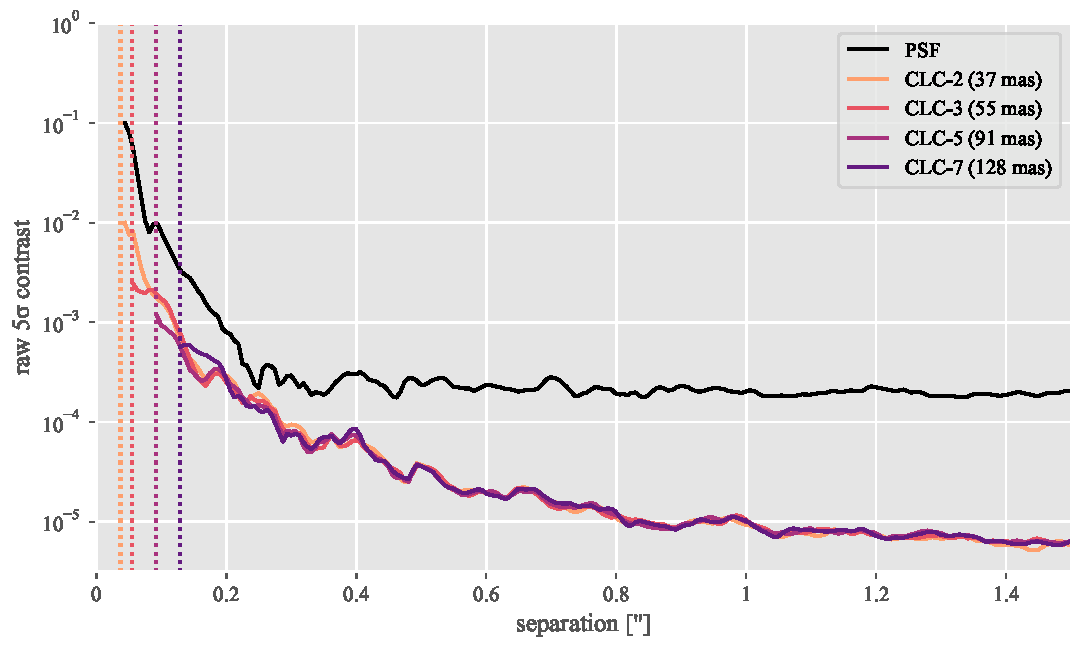
\includegraphics[width=0.9\textwidth]{figures/bench_20220526_curves}
   \caption{Raw 5$\sigma$ contrast curves measured from \qty{2}{\second} of testbed data. These curves account for small-sample statistics and have no PSF subtraction. The black curve is the non-coronagraphic contrast, while the orange through purple curves correspond to each focal plane mask. The IWA for each curve is marked with a dotted vertical line. The astrogrid speckles are masked out during the calculation, but their position is marked with a gray vertical line.}\label{fig:contrast}
\end{figure*}

\subsection{On-sky results}\label{sec:onsky}

We have not had any opportunities to use the coronagraph in good conditions for testing; most of our on-sky tests had $>$\ang{;;1.5} seeing. Our best data is from May 12, 2022 of target HIP 56083. We used a \qty{50}{\nano\meter} amplitude astrogrid with a separation of 15.5 $\lambda/D$, the same as our testbed data. An example coronagraphic image is shown in \autoref{fig:satellite-spots}b. We used 300 EM gain with 200 ms exposure times, median combining 100 frames for a total of \qty{20}{\second} of integration time. This caused significant blurring from seeing, but was necessary to achieve a high signal to noise ratio (S/N). In the future, we want to investigate further the trade-off between S/N and sharpness from shorter exposure times on coronagraphic contrast.

We constructed 5$\sigma$ contrast curves for each focal plane mask size following the same procedure as the testbed data (\autoref{fig:onsky-contrast}). Note for these observations we used a tighter field of view (256x256) which limits the max separation to \ang{;;0.75}. We used the same scaling for the satellite spot photometry as fit from the testbed data ($10^{-1.52}$) and also masked out the satellite spots. At \ang{;;0.1}, all masks have a raw contrast around $10^{-2.5}$ and drop off to \num{e-4} at \ang{;;0.75}. We expect that under better observing conditions we could achieve one to two orders of magnitude increased contrast performance with high S/N data aligned and stacked using lucky imaging for improved sharpness.

\begin{figure*}
   \centering
   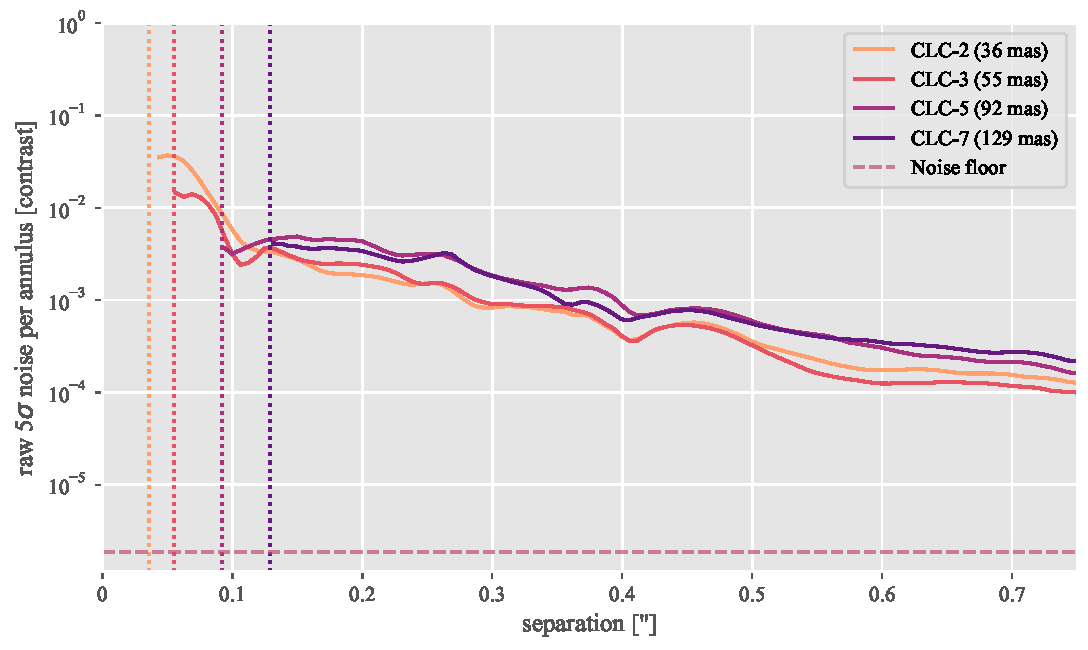
\includegraphics[width=0.9\textwidth]{figures/HIP56083_20220512_curves}
   \caption{Raw 5$\sigma$ contrast curves measured from \qty{20}{\second} of on-sky data of HIP 56083. These data were obtained on May 12, 2022 through the 750-50 filter with 300 EM gain and 200 ms exposures. The orange through purple curves correspond to each focal plane mask. The IWA for each curve is marked with a dotted vertical line. The astrogrid speckles are masked out during the calculation, but their position is marked with a gray vertical line.}\label{fig:onsky-contrast}
\end{figure*}

\section{Conclusions}\label{sec:conclusions}

In this paper we have described the design, construction, and deployment of a visible-light Lyot coronagraph on SCExAO/VAMPIRES. This coronagraph attenuates 1 to 1.5 orders of magnitude of light, greatly improving the dynamic range of the EM-CCDs used on VAMPIRES with max EM gain. Additionally, the diffraction control will improve high-contrast performance which has important applications in the optical for exoplanet science, both companion and protoplanetary disk imaging, as well as H$\alpha$ imaging. The coronagraph was approved for open-use observation starting in the 2022B observing semester.

Four partially transmissive focal plane masks were installed with IWAs of \qtylist{36;55;92;129}{\milliarcsecond}, respectively. The Lyot stop has a measured throughput of 65.7\%. During operation, the coronagraph uses ``astrogrid'' artifical speckles for photometric and astrometric calibration. We tested the coronagraph using the SCExAO internal source for characterizing the IWA, Lyot stop throughput, satellite spot relative flux, and measured contrast curves for each mask size using \qty{2}{\second} of median-combined data. The contrast was similar for each mask size, spanning \num{e-3} to \num{e-5} from \ang{;;0.1} to $>$\ang{;;0.8}. We also measured the contrast for each mask size using \qty{20}{\second} of median-combined data of HIP 56083 in poor seeing conditions. This data is highly limited by the seeing halo, but achieves raw 5$\sigma$ contrast of \num{e-2} to \num{e-4} from \ang{;;0.1} to \ang{;;0.75}.

In the future, as wavefront control improves for SCExAO, we want to explore phase-based focal plane masks such as the four-quadrant phase mask (4QPM)\cite{rouanFourQuadrantPhase2007}. Phase-based masks offer improved contrast over amplitude-based designs like the classic Lyot style, but are highly sensitive to pointing errors and thus require fine tip-tilt control for effective use\cite{huby2017}. The fine tip-tilt control is expected to improve on SCExAO during the upgrades to the facility AO system, AO 188. We are also interested in exploring apodized Lyot stops to achieve similar or improved performance in the presence of aberrations without sacrificing as much throughput.

%%%%% Appendix %%%%%

\appendix    %>>>> this command starts appendixes


\section{Code and Data Availability}\label{sec:code}

The code used for simulating the coronagraph (\autoref{sec:design}), reducing and analyzing testbed (\autoref{sec:testbed}) and on-sky data (\autoref{sec:onsky}), and for producing the figures in this paper are all available under an open-source license in a GitHub repository (\href{https://github.com/mileslucas/vampires-coronagraph}{mileslucas/vampires-coronagraph}). This code makes significant use of the Julia programming language\cite{bezanson2017} along with the open-source packages \texttt{HCIPy}\cite{por2018}, \texttt{ADI.jl}\cite{lucas2020}, \texttt{numpy}\cite{harris2020}, and \texttt{astropy}\cite{astropycollaboration2013,astropycollaboration2018}. The CAD drawings for the focal plane masks and Lyot stops are also available in the online repository. Further requests or questions about code or data are welcomed.

\acknowledgments

We wish to recognize and acknowledge the significant cultural role and reverence that the summit of Maunakea has always had within the indigenous Hawaiian community. We are most fortunate and thank the community for the privilege to conduct observations from this mountain. We would like to thank Paul Sumner for his useful advice during the construction of the Lyot stop and focal plane masks. We also thank Jonathan Williams, Thayne Currie, and Timothy Brandt for generously offering observation time to use VAMPIRES for additional characterization of the coronagraph on-sky. This work is based on data collected at Subaru Telescope, which is operated by the National Astronomical Observatory of Japan. The development of SCExAO was supported by the Japan Society for the Promotion of Science (Grant-in-Aid for Research \#23340051, \#26220704, \#23103002, \#19H00703, and \#19H00695), the Astrobiology Center of the National Institutes of Natural Sciences, Japan, the Mt Cuba Foundation and the director's contingency fund at Subaru Telescope. This research was funded by the Heising-Simons Foundation through grant \#2020-1823.

%%%%% References %%%%%

\bibliography{report} % bibliography data in report.bib
\bibliographystyle{spiebib} % makes bibtex use spiebib.bst

\end{document}
